\documentclass[a4paper]{article}

\usepackage{cite}
\usepackage
[%
left=2.54cm,% left margin
right=2.54cm,% right margin
top=2.54cm, % top margin
bottom=2.54cm,% bottom margin
a4paper% other options: a0paper, a1paper, a2paper, a3paper, a4paper, a5paper, a6paper, and many more.
]{geometry}
\usepackage{blindtext}

\usepackage[affil-it]{authblk}

\usepackage{etoolbox}
\usepackage{lmodern}

\makeatletter
\patchcmd{\@maketitle}{\LARGE \@title}{\fontsize{16}{19.2}\selectfont\@title}{}{}
\makeatother
\renewcommand\Authfont{\fontsize{12}{14.4}\selectfont}
\renewcommand\Affilfont{\fontsize{9}{10.8}\itshape}


\usepackage{lineno,hyperref}
\modulolinenumbers[5]
\usepackage{subcaption}
\usepackage{amsmath,amsfonts,amsthm}
% \captionsetup[subfigure]{position=b}

\usepackage{array}
\newcolumntype{L}{>{\centering\arraybackslash}m{3cm}}
\newcolumntype{R}{>{\centering\arraybackslash}m{2cm}}
\newcolumntype{C}[1]{>{\centering\let\newline\\\arraybackslash\hspace{0pt}}m{#1}} 
\usepackage{mathtools,amssymb}
\newcommand{\ddn}[2]{\frac{\mathrm{d}}{\mathrm{d}#1}#2}
\newcommand{\ddt}{\frac{\mathrm{d}}{\mathrm{d}t}}

\newcommand*\widefbox[1]{\fbox{\hspace{2em}#1\hspace{2em}}}

\makeatletter
\newcommand*{\rom}[1]{\expandafter\@slowromancap\romannumeral #1@}
\makeatother

\captionsetup[figure]{labelfont={bf},name={Fig.},labelsep=period}
% \captionsetup[table]{labelfont={bf},name={Table},labelsep=space}

% \usepackage{subfig}
% \usepackage[subrefformat=parens,labelformat=parens]{subfig}
\usepackage[labelformat=simple]{subcaption}		% order of subfigure with brackets
\renewcommand\thesubfigure{(\alph{subfigure})}

% \usepackage{wrapfig}
% \usepackage{lipsum}
% \usepackage{enumitem}

\usepackage{bm}					% bold and italic font



\bibliographystyle{elsarticle-num}
%%%%%%%%%%%%%%%%%%%%%%%


\begin{document}


\title{A practical a posteriori strategy to determine the optimal number of degrees of freedom for $hp$-refinement in finite element methods}
\date{\vspace{-5ex}}

\author{Jie Liu, Henk M. Schuttelaars, Matthias M\"oller}	% \corref{cor1}					% author info start from here
% \ead{j.liu-5@tudelft.nl}

\affil{Delft Institute of Applied Mathematics, Delft University of Technology, \\Van Mourik Broekmanweg 6, 2628 XE Delft, The Netherlands}

\maketitle

To improve the accuracy of solutions obtained with finite element methods, $h$-, $p$- and $hp$- refinements are widely used. They all aim at decreasing the truncation error by increasing the number of degrees of freedom (``$\text{DoFs}$'').
However, when the number of $\text{DoFs}$ becomes larger than a critical number $N_{\text{opt}} ^{(p)}$, where $p$ is the degree of the element, round-off errors accumulate and start to exceed the truncation error, and thus dominate the total error. Since further refinements will even result in less accurate solutions, the error ${Err}_{\text{min}}^{(p)}$ corresponding to $N_{\text{opt}} ^{(p)}$ is the minimum attainable error for the element of order $p$. The conceptual sketch of the dependency of the truncation and round-off error for the solution on the number of DoFs is shown in Fig.~\ref{Fig:rounding_error_p_dependent_SM_MM}\cite{LiuMH2018apractical}.

% T  is shown in .
% Both the standard and mixed FEM 

\begin{figure}[ht]
\hspace{0.2cm}
\begin{subfigure}{7.5cm}
    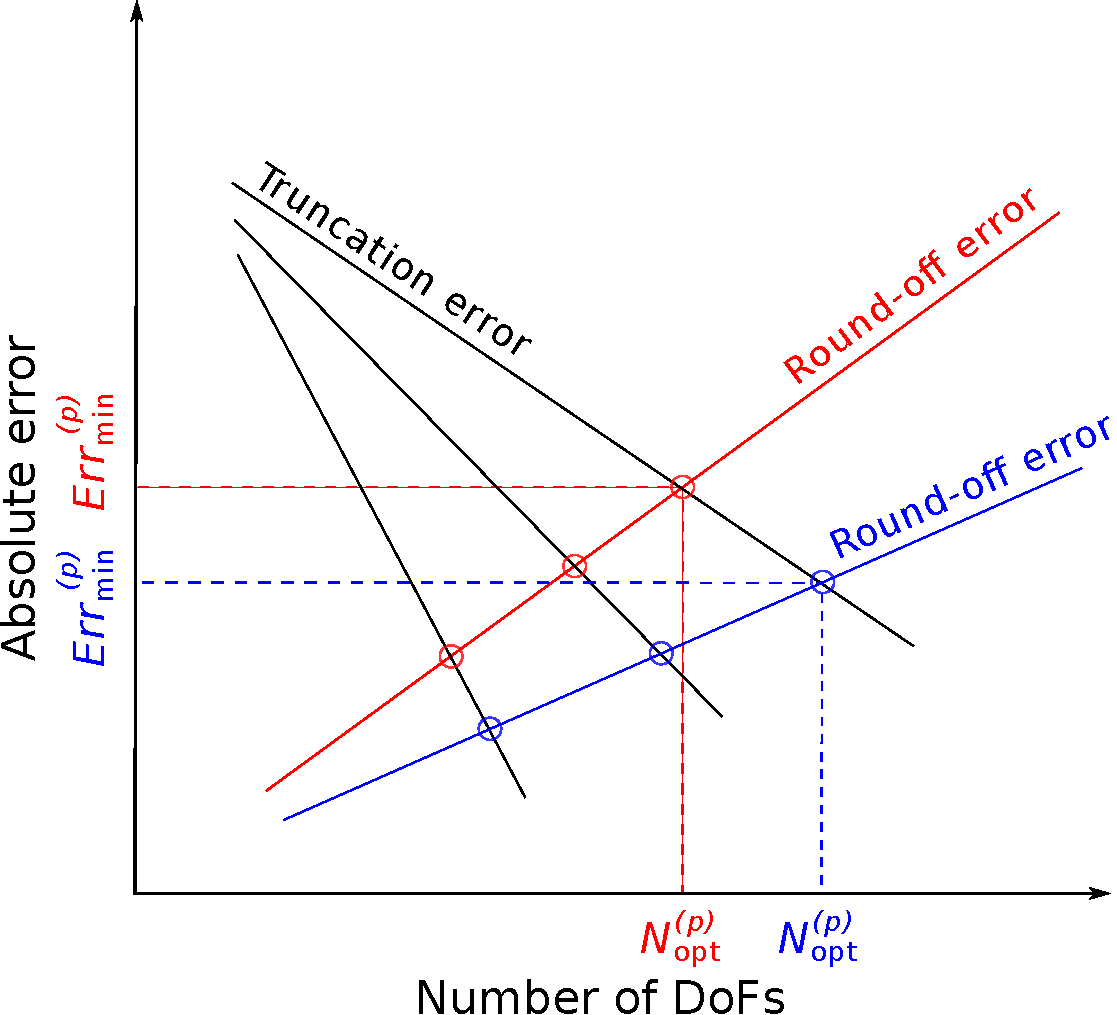
\includegraphics[width=0.9\linewidth,natwidth=500,natheight=480]{rounding_error_p_dependent_SM_MM.pdf}
    \caption{Conceptual sketch.}
    \label{Fig:rounding_error_p_dependent_SM_MM}
\end{subfigure}
\hspace{0.0cm}
\begin{subfigure}{7.5cm}
    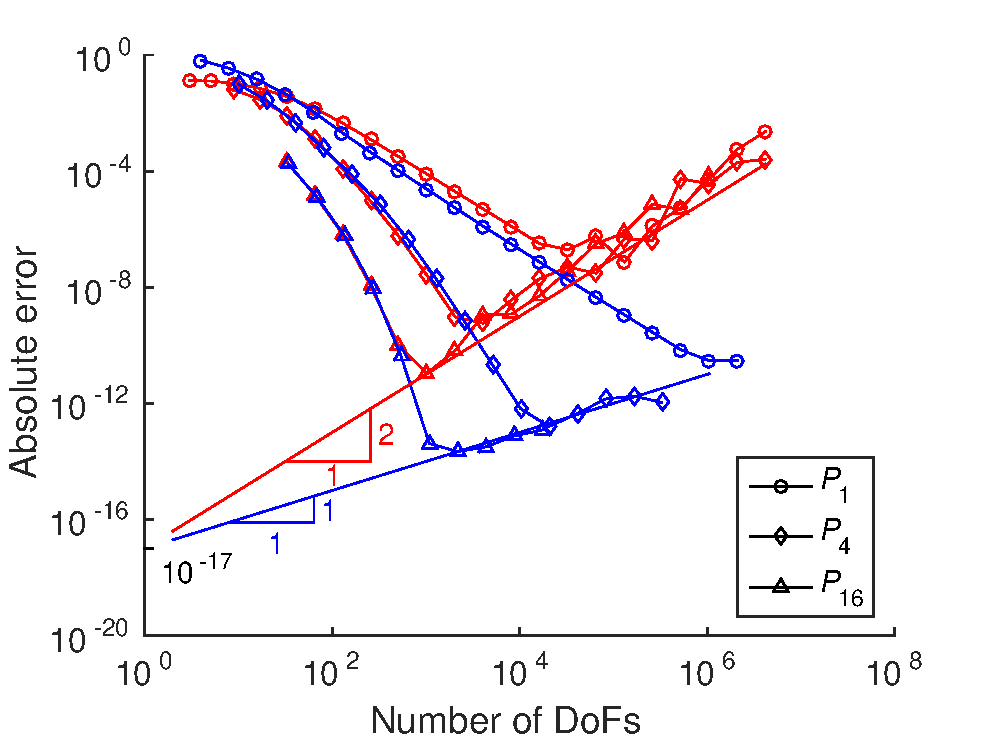
\includegraphics[width=1.2\linewidth,natwidth=500,natheight=365]{Helm_xi_S_M2_abs_solu.pdf}
    \vspace*{-5.5mm}
    \caption{Numerical results.}   
%     \subcaptionbox{Just after removal from the 3D printer plate\label{fig:MouldWithSupport}}{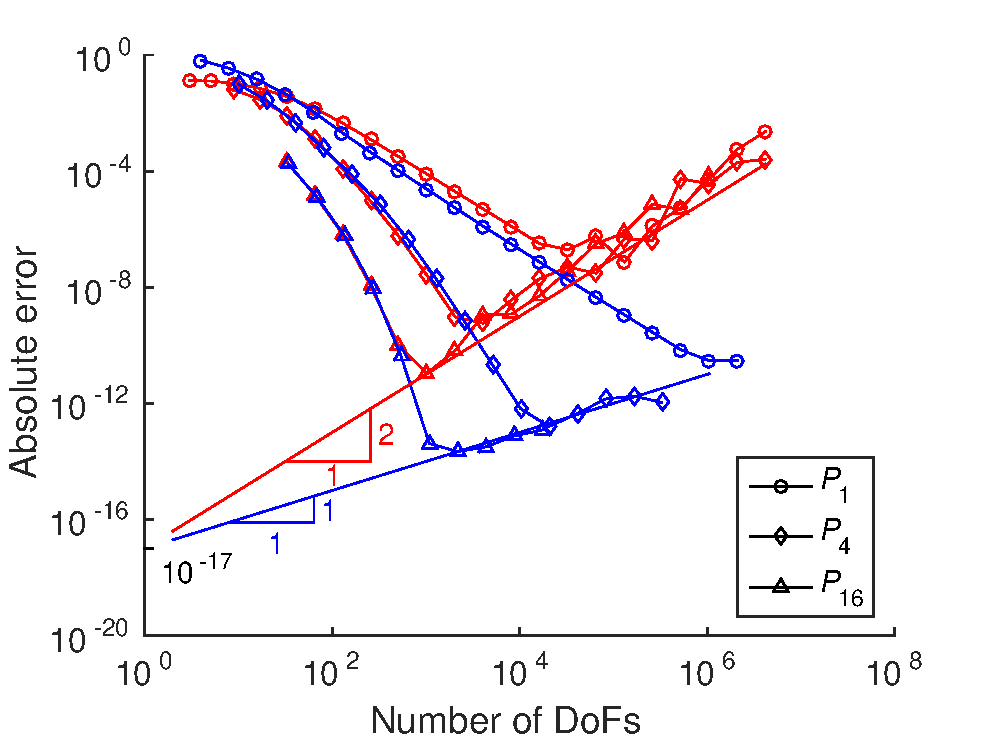
\includegraphics[width=1.2\linewidth,natwidth=500,natheight=360]{Helm_xi_S_M2_abs_solu.pdf}}
    \label{Fig:Helm_xi_S_M2_abs_solu}
\end{subfigure}
\caption{Absolute errors using the standard and mixed FEM. The red color relates to the standard FEM, the blue color relates to the mixed FEM, and the black color relates to both of them.}
\label{Fig:rounding_error_left_theoritical_right_practical}
\end{figure}

% $N_{\text{opt}}^{(p)}$ denotes the optimal number of DoFs for the element of order $p$, and 
% $\alpha_R$ denotes the offset of the line approximating the round-off error.
%  using the standard FEM and the mixed FEM,
% The truncation error decreases along straight lines, of which the slope is one order higher than the element degree. The round-off error increases along straight lines, and the lines of different elements coincide with each other. Therefore,
It shows that $N_{\rm opt} ^{(p)}$ strongly depends on $p$, with $N_{\rm opt} ^{(p)}$ decreasing for increasing $p$, both for the standard and mixed FEM.
The same trend is applied for derivative quantities.
Thus, by taking higher-order elements and the optimal number of DoFs, the best ${Err}_{\text{min}}^{(p)}$ can be achieved, resulting in most accurate solutions. 
This leads us to develop a practical a posteriori $hp$-refinement strategy that adjusts both the mesh width $h^{(p)}$ (as a function of $p$) and $p$ simultaneously so that for each $p$ the optimal mesh width $h^{(p)}_{\rm opt}$ correlates with $N_{\text{opt}}^{(p)}$.

%  the round-off errors can be reduced Fig. \ref{Fig:rounding_error_p_dependent_SM_MM}
% We also investigate the influence of the finite element formulation and demonstrate by considering several numerical examples that
% Comparing and Fig. \ref{Fig:rounding_error_inkscape_one_truncation_error_all_line_p_dependent_MM},
% Furthermore, we show that the use of the mixed-FEM approach leads to less severe round-off errors compared to the standard FEM and can, thus, yield more accurate approximations of the solution and its derivatives.
% Moreover, focusing on the one-dimensional problem, we investigate several 

To illustrate a systematic method to identify $N_{\text{opt}} ^{(p)}$ and ${Err}_{\text{min}}^{(p)}$ a posteriori, we focus on the following model problem:
\begin{equation*}
 \nabla \cdot \left(D(\bm{x}) \nabla u \right) + r(\bm{x})u(\bm{x}) = f(\bm{x}),\qquad \bm{x} \in \Omega = [0,\,1]^{\rm dim},	\label{1D_general_Helmholtz_equation}
\end{equation*}
with $u$ denoting the unknown variable, $f \in L^2 (\Omega)$ a prescribed right-hand side, $D$ and $r$ coefficient functions, and dim the space dimension.
Both the standard and mixed FEM are implemented in deal.\rom{2} \cite{alzetta2018deal}.
% the corresponding minimum attainable absolute error
% : left for the , and right for the numerical results for a 1D Helmholtz equation.
% As an example,  are shown in Fig. \ref{Fig:Helm_xi_S_M2_abs_solu}
% , with $D=(0.01+x)(1.01-x)$, $r$=-0.01$i$, $f=1.0$, $u(0)=0$ and $u_x(1)=0$.
% The absolute errors for the real part of the solution obtained with the standard and mixed FEM are shown in the left and right bound of Fig. \ref{Fig:Helm_xi_abs_solu}, respectively .
% The deal.\rom{2} finite element code \cite{alzetta2018deal} is used.


Based on an extensive numerical analysis of the one-dimensional model problem\cite{LiuMH2018apractical}, we validated the robustness of the trend in Fig. \ref{Fig:rounding_error_p_dependent_SM_MM} and have identified the possible influence factors, such as the $L_2$ norm of the solution $||u||_2$ in the standard FEM and both $||u||_2$ and the $L_2$ norm of the first derivative $||u_x||_2$ in the mixed FEM, floating-point precision, computational mesh, type and implementation of boundary conditions and choice of solvers. In particular, to make the round-off error independent of $||u||_2$ and/or $||u_x||_2$, scaling schemes for the right-hand side are put forward for both the standard and mixed FEM. 

The practical usability of the proposed $hp$-refinement strategy is demonstrated for the one-dimensional Helmholtz equation\cite{LiuMH2018apractical}, see Fig. \ref{Fig:Helm_xi_S_M2_abs_solu}, where the value of $N_{\rm opt} ^{(p)}$ is determined based on the extrapolated truncation error from coarse grid computations.
Last but not least, preliminary results show that the same trend in the one-dimensional model problem carries over to the two-dimensional one.

% Furthermore, the type of FEM method also influences the accumulation of round-off errors. That is, the mixed FEM allows for more accurate solutions, compared to the most accurate solutions obtained with the standard FEM method.
% Results on the two-dimensional problems will also be presented at that time.

% \newpage
\bibliography{mybibfile}

\end{document}